\chapter{System Design} \label{chap:design}

%\version{v1.10.2015}

\section{System Architecture Diagram}
System Architecture Diagram is a theoretic model that defines the overall view of a system. In architecture diagram we basically have defined the whole structure of a system. Android user can login/register using android application and can add and view any details like add pet profile, view pet profile, generate diet plan, alarm notification details and appointment. Added information is saved into the database and fetched from the database. While can view the information displayed on the website. Appointments can be taken through android and as well as through website user. The system architecture diagram is given below:

\begin{figure}[H]
\centering
   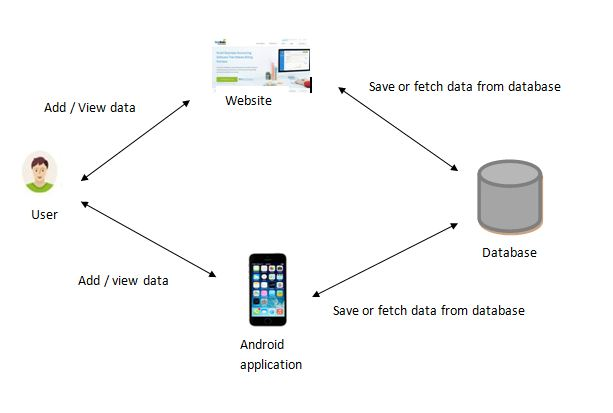
\includegraphics[scale=0.7]{4chap}
    \caption{System Architecture Diagram}
\end{figure}

\newpage
\section{Design Methodology}
Agile methodology is used to develop this project as; our requirements are incremental.

\begin{figure}[H]
  \centering
    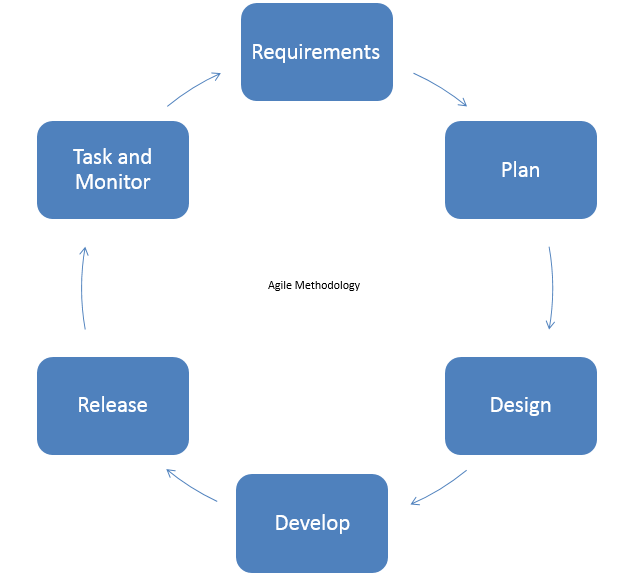
\includegraphics[scale=0.6]{Designmethod}
     \caption{Design Methodlogy}
\end{figure}



\newpage
\section{High Level Deign}
High level designs include flow charts and activity diagrams of the website and android application.

\subsection{Flow Chart}
\begin{enumerate}
\item \textbf{Flow Chart (website user)}\\
Website user first of all; will login into the system. If email and password is correct then user can only view the details available on the web application or take an appointment run time.

\begin{figure}[H]
\centering
  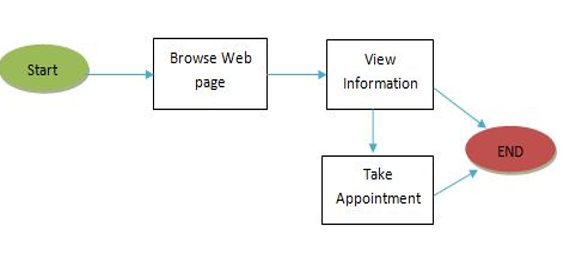
\includegraphics[scale=0.5]{figflow}
  \caption{Flow Diagram of a system (Website user)}
\end{figure}

\item \textbf{Flow Chart (Android Application user)}
\\ First of all android user will login into the system if the email and password is correct then android will be able to view details. User can add, delete and update data which is specific to pet profile. Changes in pet profile will be saved and he can fetch and re view them. Android user can take appointment or contact the doctor in case of   any emergency. Android user can log out at any time.

\begin{figure}[H]
    \centering
    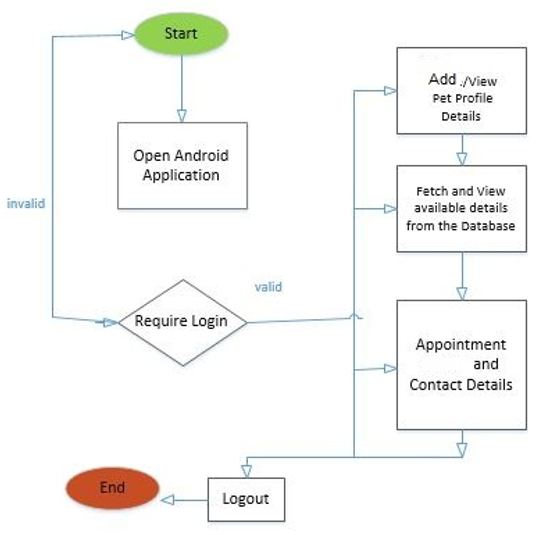
\includegraphics[scale=0.5]{figflowtwo}
    \caption{Flow Diagram of a system (Android Application User)}
\end{figure}
\end{enumerate}


\newpage
\subsection{Activity Diagrams}

\item \textbf{Activity Diagram (website user)}\\
Web user can view the details available on the web application or take an appointment at any time.
\begin{figure}[H]
\centering
   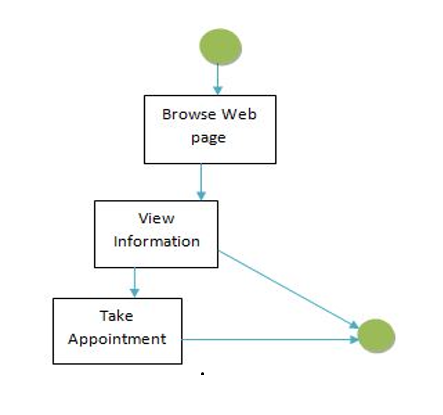
\includegraphics[0.3]{actone}
    \caption{Activity Diagram for a web user}
\end{figure}
\newpage
\item \textbf{Activity Diagram (Android Application user)}\\
\begin{figure}[H]
\centering
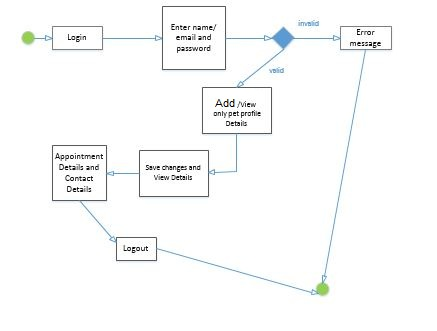
\includegraphics[0.3]{acttwo}
  \caption{Activity Diagram for an Android app user}
\end{figure}
First of all android user will login into the system if the email and password is correct then android will be to view details. User can add and view data which is specific to pet profile. User can view and generate and download the diet plans and diseases details. Android user can take appointment or contact the doctor in case of   any emergency. Android user can log out at any time.

\newpage
\item \textbf{ER Diagram)}\\
User can generate pet diet plans by selecting the correct pet specie,breed and age.User can also take an appointment and add multiple pets.User is able to view pet diseases details. 

\begin{figure}[H]
\centering
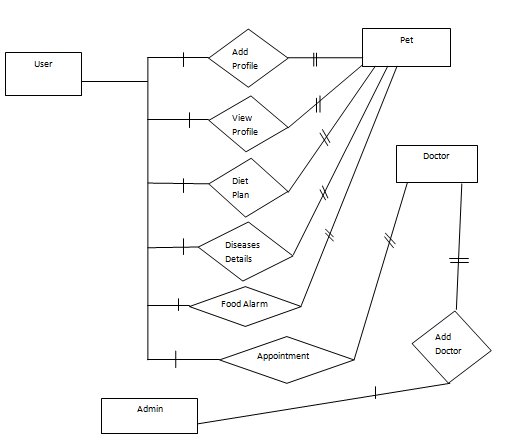
\includegraphics[0.3]{ERD}
  \caption{Activity Diagram for an Android app user}
\end{figure}








